\scanpage{86}

\inserted{Bien entendu, on pourrait en \unsure{tirer} \unsure{analogues} \deleted{\illegible{1}} ad. lib}
\inserted{le Th. 1, 1°, hypothèse b)}

\deleted{Bien entendu, \unsure{en vertu de} l'inégalité \unsure{indiquée|analogue},}
\[
\deleted{(\unsure{7|4|11})\qquad \sum\varphi(-\alpha_1,\unsure{\mathord{-}},-\alpha_n)\leq\sum\varphi(\unsure{-}\beta_1,\unsure{\mathord{-}},\unsure{-}\beta_n)}
\]

\uline{Remarque 1} Notons, \deleted{\unsure{d'ailleurs|toutefois}}, que si deux suites $(\alpha_i)_{i\leq n},(\beta_i)_{i\leq n}$ satisfont aux conditions générales du \deleted{lemme}\inserted{th. 1, 1°} \inserted{$(\alpha_1\geq\mathord{-}\geq\alpha_n,\ \alpha_1+\unsure{\mathord{-}}\alpha_M\leq\beta_1+\mathord{\cdot}\,\mathord{\cdot}+\beta_M\ \deleted{\unsure{et}}\ 1\leq M\leq n$} alors \deleted{il en est de les \unsure{mêmes suites} $(\alpha_i)_{i\leq p},(\beta_i)_{i\leq p}$ pour tout $1\leq p\leq n$, \unsure{(pourvu bien entendu que} $\sum_1^p\alpha_i=\sum_1^p\beta_i$), donc on peut leur appliquer la \unsure{formule} du lemme, et \unsure{on obtient} par \unsure{exemple} $\varphi(\alpha_1,\unsure{\mathord{-}},\alpha_p)$ qu'on obtient en remplaçant $\alpha_{p+1},\unsure{\mathord{-}},\alpha_n$ et $\beta_{p+1},\unsure{\mathord{-}},\beta_n$ par}

\inserted{suites à $k$ éléments} $(\alpha_i)_{i\leq k}$ et $(\beta_i)_{i\leq k}$ \inserted{satisfont aux conditions analogues} \deleted{quelq que soit}\inserted{quel que soit} $1\leq k\leq n$. On peut donc appliquer à ces suites le $=$ lemme, et on trouve \deleted{\unsure{donc}}\inserted{p. ex.} que \deleted{\unsure{(quitte à} \illegible{2} \unsure{le lemme}} \inserted{si $\varphi$ est une fonction convexe} croissante de \uline{$k$} arguments, on a aussi $\varphi(\alpha_1,\mathord{\cdot}\,\mathord{-}\alpha_k)\leq\varphi(\beta_1,\mathord{-}\,\mathord{-},\beta_k)$. La remarque analogue vaut pour les \deleted{corollaire 1 du lemme}\inserted{conditions du th. 1, 2°}.

\reversemarginpar
\margin{\uline{Remarque 2} Si on suppose $(\alpha_i)$ $(\beta_i)$ \unsure{comme} dans l'hyp. a, et si $f(\alpha_1\mathord{-}\alpha_n)\leq f(\beta_1\mathord{-}\beta_n)$ pour \deleted{\unsure{toute}} $f$ \unsure{tel|telle} \unsure{$\in$|que} \ldots{} alors on a $\sum_1^m\alpha_i\leq\sum_1^m\beta_i$ (évidemment, cela revenant à $\sup_H\sum_{i\in H}\alpha_i$, \deleted{\unsure{où}} $H$ à \deleted{\unsure{au plus}} \inserted{$m$ éléments})}
\margin{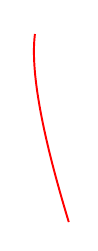
\begin{tikzpicture}[x=.01cm,y=-.01cm,baseline]\draw[red,line width=.7pt] (12,8) .. controls (4,70) and (35,181) .. (55,247);\end{tikzpicture}}
\normalmarginpar

\deleted{\uline{Applications \unsure{nouvelles de l'inégalité|et exemples de convexité} \unsure{au|du} corollaire 1.}}

Donnons maintenant un cas intéressant de fonctions $f$ satisfaisant aux conditions du \deleted{corollaire 1}\inserted{th. 1, 2°}. \deleted{\unsure{qui est}}

Si \uline{\deleted{\unsure{$f(\rho_1$}} $f(\rho_1,\mathord{-}\rho_n)$ est une fonction convexe croissante des \inserted{l'ens. des} arguments $\rho_i>0$, alors $f(e^{t_1},\mathord{-}e^{t_n})$ est \deleted{\unsure{convexe}}}\inserted{une} fonction convexe de \deleted{\unsure{chacun des arguments}} $(t_i)\in R^{n}$. Comme \deleted{la fonction convexe \unsure{sera celle qui est}} \inserted{$f$ sera} une enveloppe supérieure de fonctions \deleted{\unsure{linéaires}}\inserted{linéaires} affines \inserted{$\sum a_i x_i+\underset{\text{\unsure{qq}}}{b}$, $a_i\geq0$ (!)}, $f(e^{t_1},\mathord{-}e^{t_n})$ sera enveloppe supérieure \deleted{et que toute fonction convexe} de fonctions $\sum a_i e^{t_i}+b$, qui sont convexes (car \deleted{\unsure{si}} les fonctions $e^{t_i}$ sont convexes, et les $a_i$ positifs), donc elle sera elle-$=$ convexe.

En particulier, \deleted{si $f$ par une \deleted{fonction}\inserted{\unsure{norme}} de \unsure{Schatten}} \unsure{appelons|appl.ons}, \uline{\unsure{norme|normes} de Schatten} sur $R^n$ toute \uline{norme} $N(x)=N(x_1,\mathord{-}x_n)$ qui est symétrique, telle que $N(x_1,\mathord{-}x_n)=N(|x_1|,\mathord{-}\,\mathord{-}|x_n|)$, \deleted{et qui est fonction croissante de chacun des arguments pour} \inserted{$x_1\geq0,\mathord{-}\,\mathord{-}x_n\geq0$}, \deleted{\unsure{et par le fait est donc} \illegible{2}} \inserted{normalisée par $N(e_1)=1$.}

\reversemarginpar
\margin{
\begin{tikzpicture}[x=1cm,y=1cm,baseline]\draw[black!75,line width=1pt,line cap=round] (.02,.11)--(.27,.075)--(.53,.015);\draw[black!75,line width=.7pt,line cap=round] (.11,.025).. controls (-.015,.025) and (-.025,-.055)..(.16,-.035);\draw[red,line width=.65pt,line cap=round] (.025,.095)--(.50,.025);\draw[red,line width=.65pt,line cap=round] (.10,.055)--(.53,.01);\end{tikzpicture}}
\margin{(Alors on prouve que $N$ est fonction croissante \deleted{\unsure{des arguments}} \unsure{$(x_i)$|$(\alpha_i)$} dans \unsure{l'angle} des éléments positifs ((car la boule unité, étant stable par multiplication par une fonction $(\lambda_i)$ avec $|\lambda_i|=1$ pour \deleted{tout} $i$, le sera pour \deleted{\unsure{toute}} fonction majorée par $1$ en module).}
\margin{87}
\normalmarginpar
